\documentclass[11pt,a4paper]{article}
\usepackage[T1]{fontenc}\usepackage{lmodern}
\usepackage[margin=22mm,headheight=14pt]{geometry}
\usepackage{amsmath,amssymb,bm,booktabs,tabularx,array,graphicx,float,fancyhdr,microtype,xcolor}
\usepackage[colorlinks=true,linkcolor=blue!45!black,urlcolor=blue!45!black,citecolor=blue!45!black]{hyperref}
\setlength{\parindent}{0pt}\setlength{\parskip}{5pt}\renewcommand{\arraystretch}{1.15}
\pagestyle{fancy}\fancyhf{}\fancyhead[L]{\small QFT Project B | Step 6}\fancyhead[R]{\small Group B}\fancyfoot[C]{\thepage}
\newcommand{\dd}{\mathrm{d}}
\begin{document}\hypersetup{pageanchor=false}
\begin{titlepage}\centering\vspace*{3mm}

\includegraphics[width=36mm]{assets/bits_logo.png}\par\vspace{13mm}
{\Large\bfseries BITS PILANI K.K. BIRLA GOA CAMPUS\par}\vspace{3mm}
{\large\bfseries Department of Physics\par}\vspace{18mm}
{\LARGE\bfseries What Quantum Trace Can\\[2mm] a Heavy Particle Leave?\par}\vspace{6mm}
{\large Curvature--Spectator Entanglement\\and the Cosmological Collider\par}\vspace{10mm}
{\large\bfseries Step 6: Heavy Clock and In-in Benchmark\par}\vspace{17mm}
{\Large\bfseries Group-B\par}\vspace{5mm}
\begin{tabular}{ll}Priyansh Rawat & 2023B5A70968G\\Mayank Sinha & 2023B5A70942G\\Samarth Bhatnagar & 2023B5A70853G\end{tabular}
\vfill{\large Under Professor: Rudranil Basu\par}\vspace{7mm}{29 October 2026\par}
\end{titlepage}\setcounter{page}{1}\hypersetup{pageanchor=true}
\section{Heavy-field clock and perturbative expectation value}
Outside the horizon, discard $x^2$ terms. Integrating the light equation gives $\dot Q+g\Sigma\propto e^{-3N}$. For the decaying heavy branch, the transient can be neglected, so $\dot Q\simeq-g\Sigma$. The spectator obeys
\begin{equation}\ddot\Sigma+3\dot\Sigma+(M^2+g^2)\Sigma=0.\end{equation}
Substitution of $\Sigma\propto x^p=e^{-pN}$ yields $p^2-3p+M^2+g^2=0$. Thus
\begin{equation}p=\frac32\pm i\mu,\qquad \mu=\sqrt{M^2+g^2-\frac94}.\end{equation}
At $M=2$, $g=0.1$, $\mu=1.3266499$. A negative square-root argument gives real powers, not an oscillating clock.
The interaction-picture expansion, treating the mixed quadratic model exactly, gives
\begin{equation}\Delta\langle O(\eta_f)\rangle=-i\int_{-\infty}^{\eta_f}\dd\eta\,\langle[O_I(\eta_f),H_I(\eta)]\rangle_0.\end{equation}
For the test Hamiltonian $H_I=\gamma\int\dd^3x\,a(q')^3/3!$, the six contractions cancel $3!$. The massless derivative mode is $u'_k=Hk^2\eta e^{-ik\eta}/\sqrt{2k^3}$. The three late external modes and the factor $a=-1/(H\eta)$ reduce the time dependence to $\eta^2 e^{iK\eta}$, where $K=k_1+k_2+k_3$.

\newpage
\section{Analytic integral and numerical benchmark}
With the vacuum regulator,
\begin{equation}I_\epsilon=\int_{-\infty}^{0}\eta^2e^{(\epsilon+i)K\eta}\dd\eta=\frac{2}{[(\epsilon+i)K]^3}.
\end{equation}
The commutator selects its imaginary part. Keeping the sign from $a$ and the contractions gives
\begin{equation}B_{\rm test}=-\frac{\gamma H^5}{4k_1k_2k_3}\operatorname{Im}I_\epsilon\longrightarrow-\frac{\gamma H^5}{2k_1k_2k_3K^3}.\end{equation}
We check this independently with oscillatory sine quadrature, rather than using the analytic integral as the numerical answer. The tests use $\gamma=H=1$ and $(k_1,k_2,k_3)=(r,1,1)$ with $r=1,0.1,0.03,0.01$. At $\epsilon=10^{-3}$ the maximum relative error from the zero-regulator limit is $6.000\times10^{-6}$, comfortably below the required $0.1\%$. Agreement with the regulated analytic formula is also checked before taking the limit.
\begin{figure}[H]\centering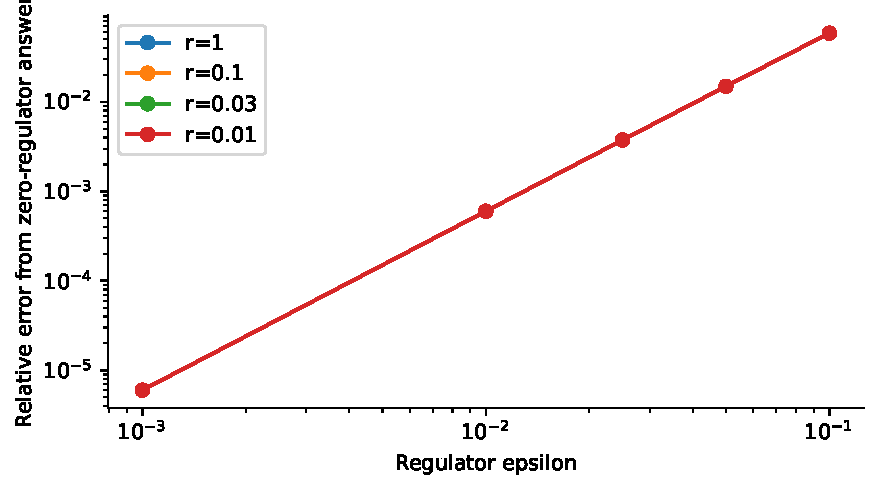
\includegraphics[width=.91\linewidth]{figures/in_in_benchmark.pdf}\caption{Regulator dependence of the independently integrated test. The curves coincide because the dimensionless relative correction depends on the regulator, not the triangle scale.}\end{figure}This fixes the overall sign, the combinatorial factor and the vacuum prescription before the spectator interaction is used. It is a Hamiltonian test; no unchecked derivative-interaction Legendre transform is assumed.\begin{thebibliography}{9}\small
\bibitem{collider} N. Arkani-Hamed and J. Maldacena, \emph{Cosmological Collider Physics}, \href{https://arxiv.org/abs/1503.08043}{arXiv:1503.08043}.\end{thebibliography}
\textbf{Code and supporting data:} \href{https://github.com/rawatpriyansh17/QFT-PROJECT-GROUP-B/tree/main/step6}{step6 on GitHub}.\newpage\section*{Contributions (equal)}\begin{center}\begin{tabularx}{\linewidth}{p{33mm}X}\toprule Member & Contribution\\\midrule Priyansh Rawat & Heavy-clock exponent and in-in derivation.\\[3mm]Samarth Bhatnagar & Sign and contraction-factor checks; benchmark review.\\[3mm]Mayank Sinha & Independent oscillatory quadrature and regulator tests.\\\bottomrule\end{tabularx}\end{center}\end{document}